\chapter{System Design and Methodology}
\section{High Level Architecture}
The architecture separates laboratory preparation from evidence recovery.
Preparation creates identifiable image states and records original marker
values. Recovery opens the selected image for reading, validates the required
structures, and writes recovered bytes and a report elsewhere. Figure
\ref{fig:architecture} shows this separation. The image passed to the reader
is an artifact of preparation; recovery never calls the embedding routine.

\begin{figure}[htbp]
\centering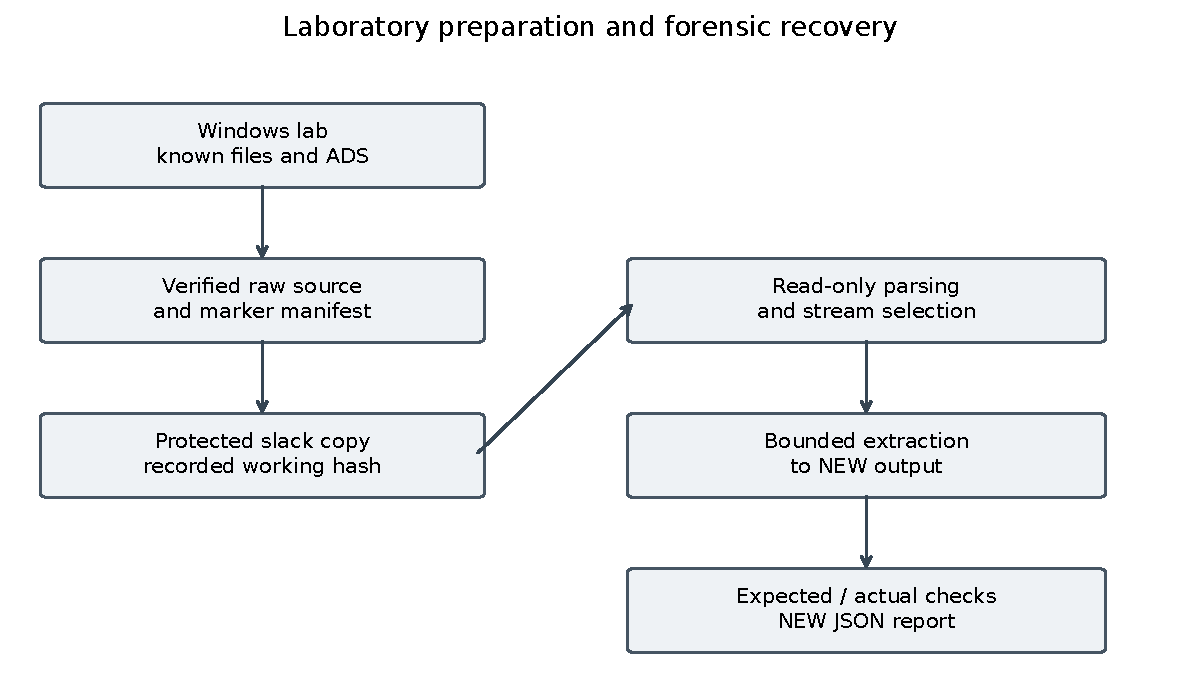
\includegraphics[width=\textwidth]{architecture.pdf}
\caption{Preparation and recovery data flow with separate output files.}
\label{fig:architecture}
\end{figure}

ADS creation took place inside the Windows guest. Slack embedding changed
only a documented range in a protected image copy. The manifest linked image
hashes, host record, payload length, offset, and original payload hash before
the later recovery comparison.

The portable fixture constructs metadata and original bytes directly so
tests can run without the large laboratory disk. Its generated expectations
remain distinct from independently recorded Windows evidence.

\section{Addressing Model and Mathematical Definitions}
Let $P$ be the NTFS partition's absolute byte offset, $B$ the bytes per sector,
$S$ the sectors per cluster, $C$ the cluster size, $L$ a logical cluster
number, and $R$ the MFT record size. The implementation uses:
\begin{align}
C &= B S,\\
O_{\mathrm{cluster}} &= P + LC,\\
O_{\mathrm{MFT}} &= P + L_{\mathrm{MFT}} C,\\
O_{\mathrm{record}}(n) &= O_{\mathrm{MFT}} + nR.
\end{align}
The last equation assumes supported contiguous MFT storage. Recovery checks
that assumption instead of treating it as valid for arbitrary images.
The metadata reader's simpler selected-record path has a narrower validation
guarantee, as discussed in Chapter 6.

For the Windows laboratory, $P=1{,}048{,}576$, $C=4{,}096$, and
$L_{\mathrm{MFT}}=786{,}432$, giving
$O_{\mathrm{MFT}}=3{,}222{,}274{,}048$. These are measured properties of the
controlled image, not universal NTFS constants. The generated fixture instead
uses 512-byte clusters and a much smaller MFT location.

For a nonempty ordinary stream of logical size $F$, final-cluster slack has
length
\begin{equation}
Q = (C - (F \bmod C)) \bmod C.
\end{equation}
If $Q=0$, there is no final-cluster tail to select. For a fragmented file,
the final logical cluster must be resolved through the run sequence. Adding
$F$ to the first physical extent is valid only when that extent actually
contains the relevant logical position. The tests include a negative LCN
delta so this distinction is exercised rather than assumed.

If $A$ is the absolute start of the final physical cluster containing
logical content, slack begins at $A+(F\bmod C)$ when the remainder is nonzero.
For the laboratory document, $F=13{,}437$ and $C=4{,}096$, so the remainder
is 1,149 and $Q=2{,}947$. The selected marker starts at byte 16,049,277.
A request with relative slack offset $d$ and length $N$ must satisfy
$d\geq0$, $N>0$, and $d+N\leq Q$.

Capacity is reported in bytes and bits for this storage carrier. Occupancy
is $100N/Q$ percent of the available final-cluster tail, not bits per pixel.
For the 25-byte laboratory marker this is approximately 0.8483\% of the
2,947-byte tail. That percentage is measured use of this location, not a
maximum ADS capacity or a filesystem-wide concealment rate.

\section{Embedding Algorithm}
The manual ADS procedure writes the known marker to the named stream
\file{hostfile.txt:CapstoneEvidence}, measures its exact length, and records
its hash. The host path and stream name are part of the experiment's identity.
No assumption is made that reading the unnamed host stream retrieves the ADS.

The controlled slack-copy algorithm is summarized below. It is deliberately
more restrictive than a general disk editor: the source must match the known
laboratory image, the chosen record must represent a supported file, and
the destination must be new.
\begin{lstlisting}
require source hash equals documented lab hash
require destination is new and distinct from source
read partition, boot geometry, record, and restored attributes
require one supported unnamed nonresident data stream
decode runs and calculate final logical cluster and slack
require marker fits entirely inside that final-cluster tail
copy source to destination; change only selected marker bytes
compare complete copy with source plus intended marker range
save source hash, copy hash, marker hash, and location manifest
\end{lstlisting}
The complete comparison supports a specific preservation claim: all bytes
outside the designated range match the source. It does not claim that the
working image itself is unchanged, because embedding intentionally changes it.
Recovery integrity is evaluated later, relative to that working image.

\section{Extraction and Verification Algorithms}
Extraction first selects the content's identity and then copies its bytes.
The identity is a record number and exact stream name, with an optional
slack-relative selection. This prevents an empty or default stream name from
silently standing in for the requested ADS.
\noindent\begin{minipage}{\linewidth}
\begin{lstlisting}
validate image geometry and supported MFT coverage
read selected record; validate flags and sector-tail fixups
parse attributes; reject unsupported extensions or stream flags
select exactly one DATA stream with requested name
if resident: use value from restored record
otherwise: decode runs in logical order and validate bounds
if slack requested: resolve final cluster and bound selected range
require source, output, and report paths are distinct
require output and report do not already exist
hash source before extraction; export to new output
compare output length/hash with independently supplied expectations
hash source after extraction; save result and errors
\end{lstlisting}
\end{minipage}

For ordinary nonresident streams, export is limited to initialized content
followed by zero bytes up to logical end where required. It does not append
slack. A slack request is an explicit alternate selection with its own length
and a report field preserving the host's logical size. This allows the
reviewer to distinguish a 25-byte recovered marker from a 13,437-byte host.

Verification has three separate comparisons. The expected-image comparison
identifies the selected source when an expected image hash is supplied.
The before/after comparison checks observed source preservation during the
run. The recovered-payload comparison checks expected content and size.
These comparisons address different failure modes; none should be described
simply as an undifferentiated hash match.

\section{Report Schema and Selection Metadata}
No custom network protocol or embedded packet header is used. The markers
are plain byte strings, and the metadata needed to find them is supplied
through manifests and CLI parameters. Table \ref{tab:schema} describes the
report fields that play the relevant coordination role. Their lengths are
not represented as fixed binary header sizes because the report is JSON.

\begin{table}[htbp]\centering\small
\caption{Verification report fields and their interpretation.}\label{tab:schema}
\begin{tabular}{p{2.15in}p{3.8in}}\toprule
Field & Interpretation\\\midrule
\file{record_number}, \file{stream_name} & Selected metadata identity.\\
\file{recovery_kind} & Ordinary stream or bounded slack payload.\\
\file{extents} & Absolute byte ranges used for a nonresident export.\\
\file{host_logical_size} & Host size retained for a slack selection.\\
\file{expected_length}, \file{expected_sha256} & Independent payload expectations.\\
\file{recovered_length}, \file{recovered_sha256} & Measured output values.\\
\file{source_image_hash_match} & Agreement with supplied expected image hash.\\
\file{source_unchanged} & Agreement of source hashes before and after export.\\
\file{overall_result}, \file{errors} & Decision and diagnostic information.\\\bottomrule
\end{tabular}\end{table}

\section{Security Model}
The examiner is assumed to possess an authorized stable image and a trusted
expectation manifest. An adversary may know the hiding method, observe the
plaintext markers, or alter accessible storage bytes. No secret key prevents
them from reading a known marker. The trust boundary is therefore around
evidence preservation and the provenance of expectations, not cryptographic
confidentiality.

Malformed metadata should be refused. Before/after hashing neither locks
the source nor proves its creator; stable preserved storage remains an
operational assumption.

\section{Experimental Design}
Three evidence layers are used. Historical Windows checks establish image
geometry, eight file lengths, and the two marker recoveries. Automated tests
exercise valid and invalid structures in small inputs. The final report
campaign constructs 50 slack payloads: ten deterministic samples at each
of 1, 25, 100, 200, and 324 bytes in a 324-byte synthetic slack region.
The random seed is fixed at 4,812,026 so the bytes can be regenerated.

Each sample is first recovered unchanged and compared byte-for-byte with
its separately written original. The baseline independently reads the known
construction offset without parsing metadata. A second new image changes
one bit in the first payload byte; recovery uses the changed image's correct
hash but retains the original payload expectation. This isolates payload
integrity failure from wrong-image identification. It is not an experiment
in attack-resistant concealment.

Bit error rate is defined as
\begin{equation}
\mathrm{BER}=100\frac{\sum_{i=1}^{N}\operatorname{popcount}(x_i\oplus y_i)}{8N}\%.
\end{equation}
Clean exact matches should have BER zero. One changed bit should yield
$100/(8N)$ percent and a failed payload comparison. Timing values are
recorded for single in-process runs on tiny cached inputs, with reporting
and hashing included for the structured path. They are not storage-throughput
benchmarks.

\subsection{Detection and Evasion Experiment}
A separate November 25 experiment applies two fixed screening rules to
100 newly constructed images, using seed 4,811,125. The ADS rule flags any
named data stream in the selected record. The slack rule searches the
entire calculated final-cluster tail for the known 25-byte marker; it does
not receive the planted offset. Neither rule receives the construction
label or an expected payload hash. This evaluates discovery rules rather
than reusing recovery-integrity decisions as detection results.

The ADS group contains 25 intentionally hidden named streams, ten legitimate
named-stream controls, and 15 ordinary-file controls. The slack group contains
15 plaintext markers, ten reversibly XOR-transformed markers, 15 random-tail
controls, and ten controls containing the marker only in logical file data.
The XOR transformation changes each marker byte with constant \file{0x5A};
it is a simple signature challenge, not encryption or a claim of strong secrecy.
Labels are assigned by construction before either detector runs. All images
share one synthetic layout; they are not independent Windows-formatted volumes.

For intentionally hidden content as the positive class, define true positives
($TP$), false negatives ($FN$), false positives ($FP$), and true negatives
($TN$). A legitimate named stream flagged for review is an $FP$ relative to
this hidden-content label, even though its stream enumeration is correct.
The following percentages use separate denominators for each rule:
\begin{align}
\mathrm{Accuracy} &= 100\frac{TP+TN}{TP+TN+FP+FN},\\
\mathrm{Detection} &= 100\frac{TP}{TP+FN},\\
\mathrm{FPR} &= 100\frac{FP}{FP+TN},\\
\mathrm{Evasion} &= 100\frac{FN}{TP+FN}.
\end{align}
Evasion means a hidden-positive case missed by that particular rule.
Malformed inputs abort the experiment rather than being counted as clean
negatives. Before/after SHA-256 checks verify that screening preserves each
source. The Windows image supplies two additional known-positive checks,
not a real-volume negative-rate estimate.
